\chapter{Datasets and Data Preparation}\label{ch:datasets}
\section{Selection principles and evidence levels}
The repository contains demonstration media but no labelled research dataset. Data acquisition was therefore part of the experiment. Selection prioritised reachable public files, variation relevant to the application, ground truth appropriate to the measured task, and a subset size compatible with the available host. Two complementary public collections were selected: HPatches for planar geometric evaluation and Tokyo query photographs for real cross-time place recognition. A generated set adds controlled photometric perturbations.

These collections supply different evidence levels. A labelled place identity establishes whether a retrieved record refers to the intended location. A homography establishes a planar pixel mapping. A calibrated camera pose and three-dimensional map would establish metric localisation error. The first two are present in the selected data; the third is not. The report does not infer missing ground truth from visual plausibility, GPS labels or a fitted matrix.

\resultinput{datasets.tex}
\Cref{tab:datasets} summarises the actual evaluation collections. The downloaded and generated image counts come from the data and preparation manifests. The HPatches archive was downloaded in full from the author's reachable mirror, while only selected sequences were extracted for evaluation. Tokyo images were retrieved as selected ZIP members using byte ranges; their complete metadata records were retained to make the selection rule inspectable. Download failures and the bounded full-archive attempt are preserved in the command journal.

\section{HPatches subset}
\subsection{Acquisition and deterministic selection}
The original HPatches host failed DNS resolution during the recorded download check. The dataset author's Hugging Face mirror was reachable and supplied the full sequence archive. The manifest records its URL, file hash, extracted-image hashes and per-sequence file counts. This distinguishes a verified local copy from a statement that a URL happened to exist when the thesis was written.

The selected evaluation set consists of the first twelve sequence names in lexicographic order for each of the illumination and viewpoint prefixes. Every selected sequence contributes its reference image, all five targets and their corresponding homography files. Thus \HpImages{} images and \HpPairs{} reference-target pairs are evaluated. The choice uses names and metadata before inference, rather than selecting pairs on which one method appears stronger.

The images are resized only when loaded by the common I/O module. Original homographies remain unmodified on disk. Their transformation into the working-image coordinate convention is computed during evaluation. This avoids creating a second ambiguous ground-truth directory whose matrices might no longer correspond to the original files. \ifFullReport The exact selected names are listed in \cref{app:structure}.\fi

\subsection{Illumination and viewpoint protocols}
The two prefix groups are evaluated separately because they probe different failure mechanisms. Illumination sequences change the appearance of a scene while retaining a related view. Viewpoint sequences change the projective relationship and visible detail. The official dataset description motivates this distinction \citep{balntas2017,hpatchesrepo}. No attempt is made to relabel every illumination pair as a day/night pair: the prefix is the authoritative task label available for this experiment.

For matching, each target is paired with its own sequence reference. For the custom retrieval task, the gallery contains one reference from every selected sequence, and a target's correct identity is its sequence name. This provides distractors and a reproducible image-retrieval exercise. It does not add geographic coverage or convert HPatches into a city-scale VPR benchmark. Related targets from one sequence also remain statistically dependent, which motivates clustered uncertainty estimates.

\subsection{Rights and source attribution}
HPatches combines sequences with source-specific attribution described by its maintainers. The repository's software licence should not be assumed to grant a blanket commercial licence for all imagery. The artifact retains source links and uses the data as a research input. Any distribution of extracted photographs or a public product built from them requires review of the original source terms. This limitation is documented rather than replaced with an unsupported ``open data'' label.

\section{Tokyo cross-time subset}
\subsection{Available archive and labels}
The accessible Tokyo archive contains camera-phone query images and CSV metadata. The metadata identifies image filenames, geographic positions, viewing-direction labels and capture-condition labels. The original dataset was introduced for place recognition under time-of-day and viewpoint change \citep{torii2015}. The public query URL was confirmed through the dataset-formatting documentation \citep{tokyodownload}.

A direct full-archive transfer exceeded the chosen bounded timeout and was not treated as a successful dataset download. Instead, the downloader read the ZIP central directory and retrieved required members with HTTP byte ranges. It checked the decompressed size and the archive's CRC for each member before writing it. SHA256 fingerprints were then recorded for future reproduction. Partial archive files are not used as valid complete archives.

All available CSV members were downloaded before subset selection. Records were grouped by their exact latitude-longitude site key. A complete selected site needed a front-facing daytime image, a left-facing daytime image, a front-facing night image and a front-facing sunset image. The first \TokyoSites{} complete site keys in lexicographic order were retained. That produces \TokyoImages{} image files with a transparent, metadata-only selection rule.

\begin{figure}[htbp]\centering
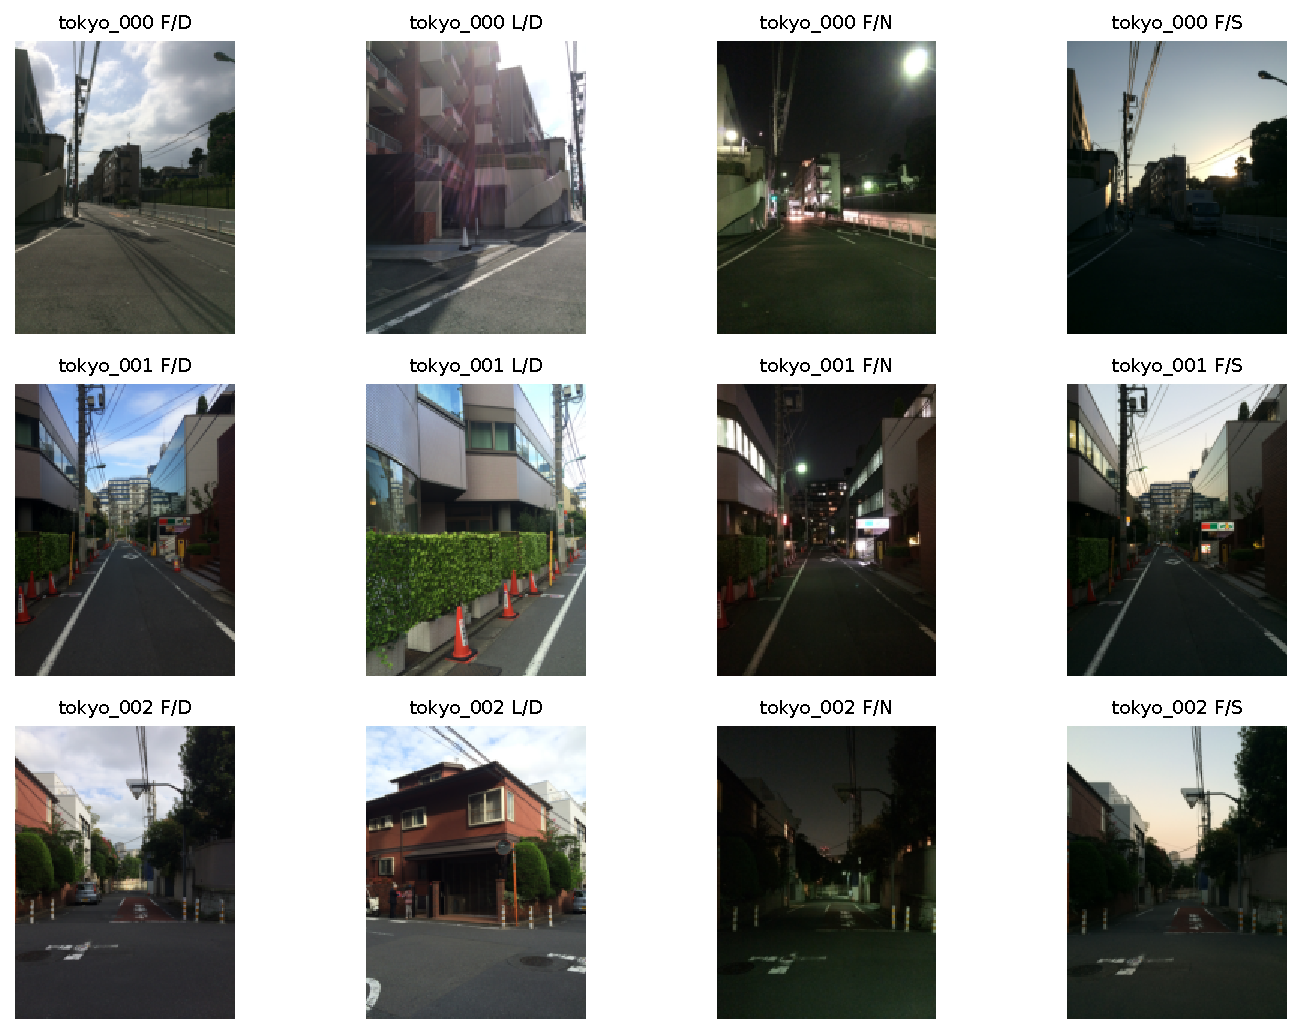
\includegraphics[width=\textwidth]{tokyo_contact.pdf}
\caption{Actual downloaded photographs from the first selected Tokyo sites. Columns follow the retained front/day, left/day, front/night and front/sunset records. Orientation and condition labels come from the source metadata.}\label{fig:tokyo-data}
\end{figure}

\Cref{fig:tokyo-data} illustrates the resulting condition coverage. Visual inspection confirms that the retained night examples are real night photographs rather than images created by gamma correction. It also shows that a left-facing daytime observation can depict substantially different scene content from the front-facing gallery image. This makes the day-to-day split a viewpoint stress test, not necessarily an easier control than the aligned cross-time pairs.

\subsection{Reference-to-query direction}
Condition names throughout the artifact follow the arrow from reference to query. Day-to-night uses a daytime front reference and a night front query. Night-to-day reverses those roles. Day-to-sunset uses a daytime front reference and a sunset front query. Day-to-day uses a daytime front reference and a daytime left query. There is one query per selected site in each of these protocols.

The gallery has one reference per selected site. Place correctness uses the stored site identity, not a distance threshold inferred after observing predictions. The reverse protocol is useful because extraction and matching may not behave symmetrically when query and reference roles change. It nevertheless reuses the same physical sites, so the protocols are related observations rather than independent geographic test sets.

\subsection{Difference from the official benchmark}
The official Tokyo retrieval task uses a street-view image database. The executed protocol uses query photographs as a small cross-time reference gallery. This changes database scale, appearance distribution, viewpoint alignment and distractor difficulty. Results are therefore labelled ``Tokyo cross-time subset'' throughout the thesis. They must not be compared directly with published official benchmark recall values.

The restriction is scientifically important when recall saturates. A small gallery with aligned front-facing views can be easy even though night recognition is difficult in a larger operational setting. Conversely, a deliberately different viewing direction can reduce overlap despite unchanged time of day. The experiment identifies these task properties rather than treating all appearance labels as a fixed difficulty ordering.

The query archive does not provide the calibrated camera poses or per-pair homographies needed for metric localisation or true planar-accuracy scoring. GPS site labels support recognition evaluation only. Geometric acceptance is reported, but a successful fitted homography is not assigned a metric translation error. The missing pose criteria are explicitly listed as unavailable in the results.

\section{Synthetic appearance and camera perturbations}
\subsection{Source images and identity semantics}
The synthetic set contains transformations of both repository images and selected HPatches references. Repository filenames do not establish independent real-world places. Their labels are therefore source-image identities. Retrieving a transformed \code{reference.jpg} means recognising its source image, not proving that the system has generalised to a new geographic location.

Six source images are transformed under five conditions and three fixed seeds, giving \SyntheticQueries{} generated queries. The gallery includes additional HPatches references as distractors. Every generated query has a known source identity and a known reference-to-query homography. The preparation manifest records the generated file hashes, seeds and benchmark-manifest hash so the exact test inputs can be regenerated and checked.

\subsection{Photometric operations}
The daytime condition changes brightness within a bounded range. Night conditions apply a gamma curve, reduced gain and additive noise. The severe condition uses a stronger attenuation; a warm-night condition additionally changes channel gains. The fog-like condition blends a bright low-contrast component and applies mild blur. These are explicit stressors, not calibrated physical camera or weather models.

\begin{figure}[htbp]\centering
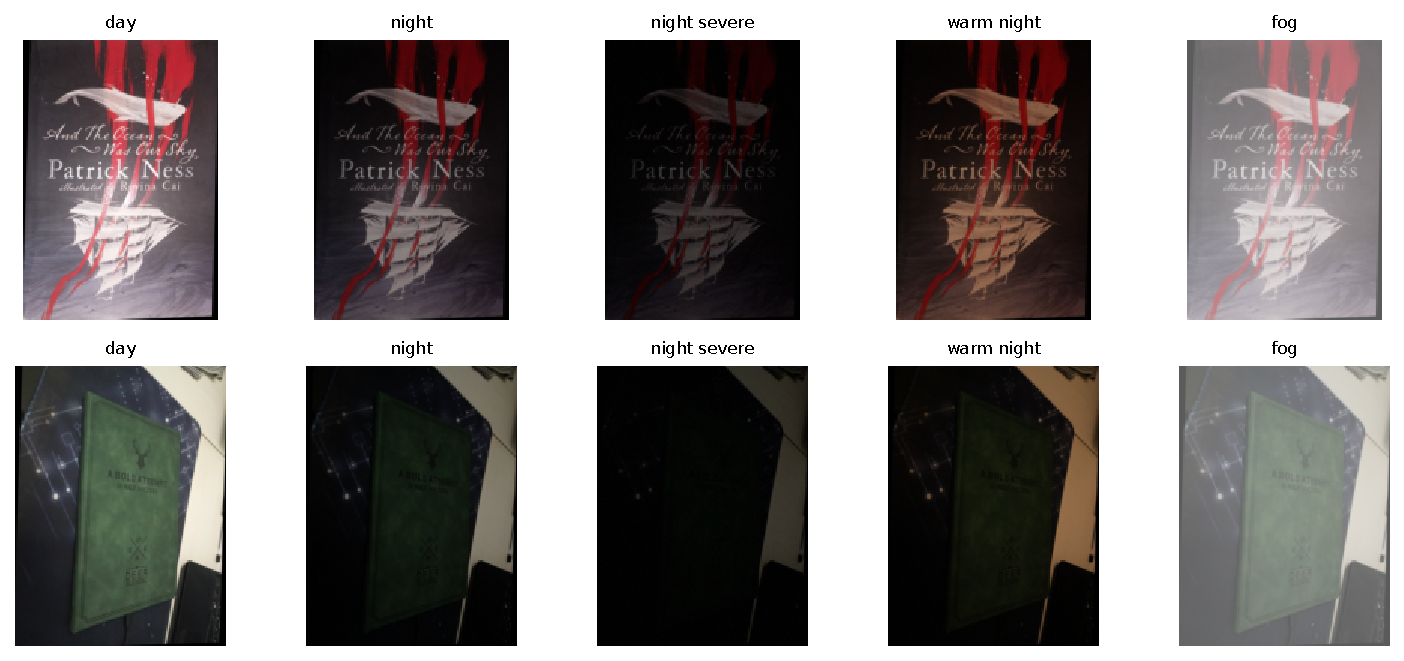
\includegraphics[width=\textwidth]{synthetic_contact.pdf}
\caption{Actual seeded synthetic queries generated from the two repository images. Columns show the evaluated photometric conditions. ``Fog'' denotes a contrast-and-blur simulation, not a real weather capture.}\label{fig:synthetic-data}
\end{figure}

\Cref{fig:synthetic-data} provides an audit of their visual effect. The operations preserve scene geometry and do not introduce night-specific light sources, glare, moving objects or seasonal occlusion. Additive noise is not a full sensor noise model. A good result here establishes tolerance to these implemented perturbations only. Real Tokyo images provide a separate, narrower check under natural temporal appearance change.

\subsection{Known geometry and deterministic seeds}
Before appearance modification, a small random projective warp perturbs the image corners. The seed determines both this warp and the subsequent photometric randomness. The homography is stored explicitly, including the scale mapping from the original reference to the working-resolution source. This detail prevents a synthetic experiment from accidentally comparing an estimate in resized coordinates with a ground-truth matrix in original coordinates.

The three query seeds support repeatability and sensitivity analysis. They do not create three independent physical scenes. Confidence statements must therefore preserve source identity as a grouping variable. Likewise, increasing the number of augmentations does not compensate for the small number of base photographs. The thesis reports those dependencies as validity constraints.

\section{Training and evaluation separation}
The optional adaptation experiment reserves the first four illumination and first four viewpoint sequences for training the projection head. Remaining selected sequences form the held-out HPatches retrieval evaluation. Training never uses Tokyo photographs. Additional synthetic training perturbations use a separate fixed seed list. The backbone remains frozen, and no test-based checkpoint selection is performed.

The main pretrained comparison may evaluate all selected HPatches sequences because none is used to train the supplied models within this artifact. The adaptation table uses only its held-out identities. Its numbers should therefore be compared with the pretrained descriptor reevaluated on that same held-out subset, not with a main-table average over a different set. The scripts preserve both denominators to prevent that drift.

\section{Open-set diagnostic}
An additional diagnostic uses HPatches images as unknown queries against a Tokyo gallery. These images have no valid place identity in that gallery. A retrieval system still returns a ranking, but an anchoring system should reject all candidates unless there is sufficient evidence. The diagnostic reports acceptance as an error condition; retrieval recall is not meaningful when no correct gallery identity exists.

The collection-level difference makes this a limited open-set test. It does not represent a difficult nearby look-alike building, malicious image replay, or two nearly identical store fronts. Its purpose is to verify that the pipeline can return no anchor and to expose gross false acceptance. More realistic negative data are required before using the measured rejection behaviour as a safety assurance.

\ifFullReport
\section{Larger benchmarks not included}
Official Aachen, RobotCar and Extended CMU documentation and download locations were inspected. Their image and mapping archives were not downloaded for the executed comparisons. The choice reflects the already bounded laptop experiment and the additional mapping, calibration and evaluation work needed to report pose metrics correctly. They are not described as universally inaccessible or as requiring registration when the recorded sources were publicly reachable.

MSLS was inspected as a route to broader seasonal and sequence coverage. Its official repository points to its current download site and describes relevant subtasks \citep{warburg2020}. No MSLS images were included. Pittsburgh, SF-XL, Oxford/Paris and Google Landmarks were candidate alternatives rather than attempted downloads in this run. The artifact makes no statement that these untested candidates failed to download. Exact manual locations and expected layouts for the principal missing benchmarks are provided in \cref{app:reproduction}.
\fi

\section{Integrity and idempotent acquisition}
The downloader validates both archive-derived member properties and locally recorded hashes. Repeated execution checks existing files and skips a valid collection. Missing data can be restored and checked against the pinned manifest; an existing corrupt file produces an explicit error instead of silently changing the input. Archive paths are not extracted blindly: selected basenames and sequence directories determine destinations.

File-count checks enforce the expected image and homography structure. The final \code{benchmark.json} freezes protocol definitions before inference, and its hash is recorded with the run configuration. These controls do not prove that the original benchmark labels are error-free, but they establish exactly which input bytes and label rules produced the thesis results.
